

\section{Inclinação}
\label{inclinacao}

 
\begin{table}[ht!]

	\begin{tabular}{r l|l p{12cm} }
		
		\textcolor{gray}{Especificação} &&& 	{Sensor de Inclinação analógico }\\
		\textcolor{gray}{Data} &&& 				{24/06/2014}\\
        \textcolor{gray}{Beneficiado} &&&		{IFM} \\
        \textcolor{gray}{CNPJ} &&& 				{02.263.430/0001-21} \\
        \textcolor{gray}{Número Nota} &&& 		{92766} \\
		\textcolor{gray}{Quantidade} &&& 		{4} \\
		\textcolor{gray}{Valor} &&& 			{R\$1.088,97 + 3.266,93} \\
		\textcolor{gray}{Data Sheet} &&& 		{Anexo VII - \ref{datasheet_inclinacao} }
		\\

		\textcolor{gray}{Função no projeto} &&& {O sensor de inclinação é responsável
		por indicar o ângulo de inclinação da viga pescadora.}
		\\
		\textcolor{gray}{Razão da Escolha} &&& {Menor custo e grau de proteção IP67.}
		\end{tabular}
\end{table}

\newpage
\subsection{Foto do Material}
\begin{figure}[H]
 \centering
 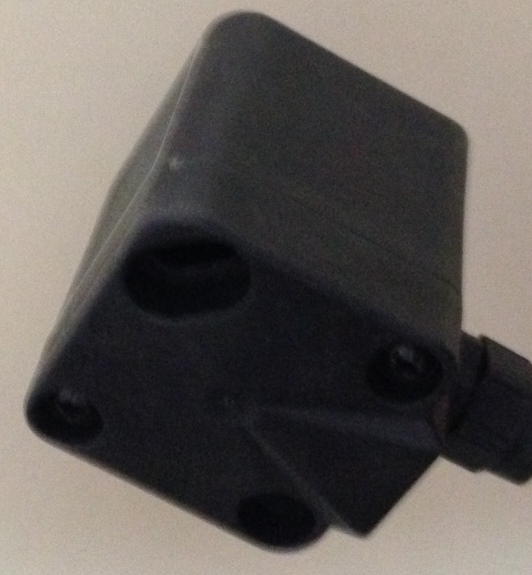
\includegraphics[width=1\columnwidth]{Inclinacao/foto.jpg}
 \caption{Sensor de Inclinação}  
\end{figure}

\subsection{Nota Fiscal}
\begin{figure}[H]
 \centering
 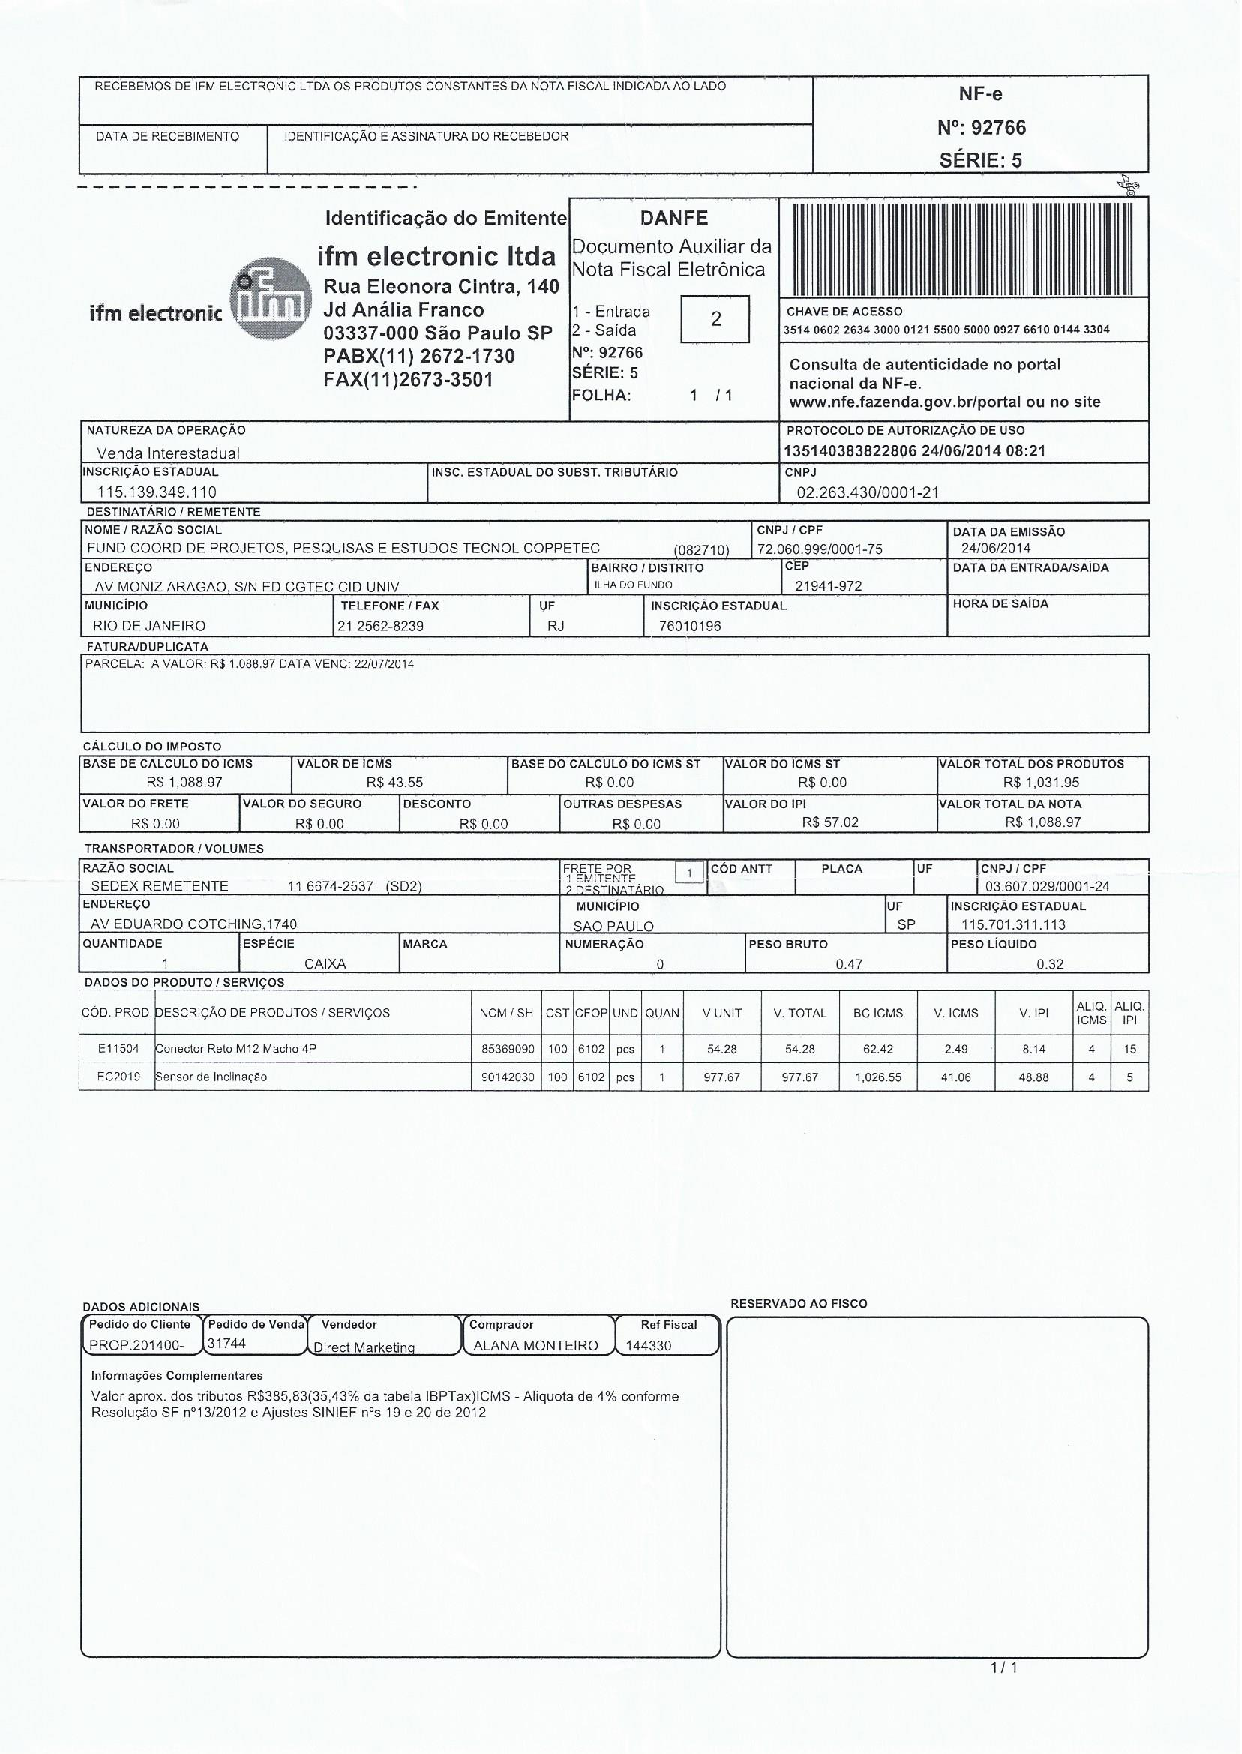
\includegraphics[width=1\columnwidth]{Inclinacao/nota_ifm1.pdf}
 \caption{Nota Fiscal do sensor de inclinação}
 \end{figure} 
 
 \subsection{Nota Fiscal 2}
\begin{figure}[H]
 \centering
 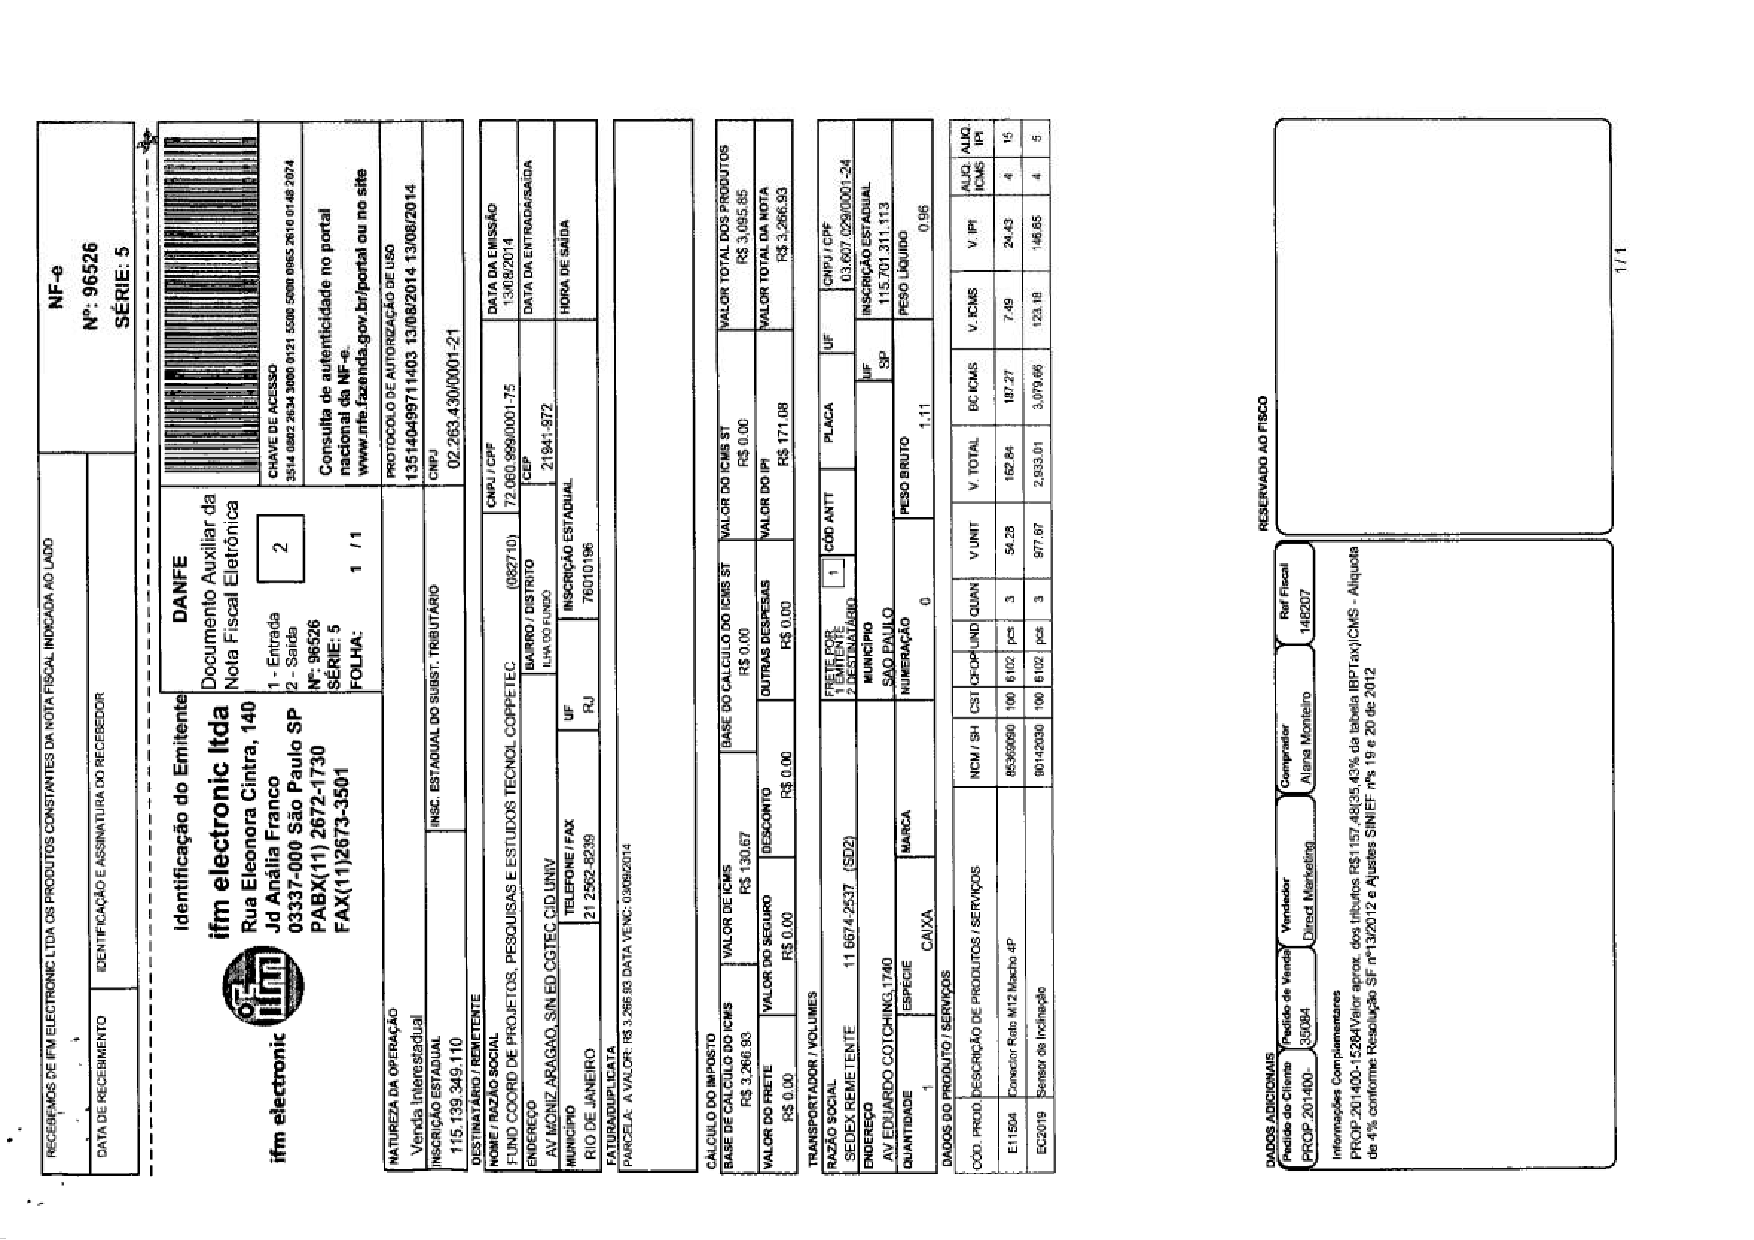
\includegraphics[width=1\columnwidth, angle=270 ]{Inclinacao/nota_ifm2.pdf}
 \caption{Nota Fiscal 2 do sensor de inclinação}
 \end{figure} 